\documentclass[11pt,preprint, authoryear]{article}

\pagestyle{plain}

\usepackage{lmodern}
%%%% My spacing
\usepackage{setspace}
\setstretch{1.5}
\DeclareMathSizes{10}{12}{8}{8}

% Wrap around which gives all figures included the [H] command, or places it "here". This can be tedious to code in Rmarkdown.
\usepackage{float}
\let\origfigure\figure
\let\endorigfigure\endfigure
\renewenvironment{figure}[1][2] {
    \expandafter\origfigure\expandafter[H]
} {
    \endorigfigure
}

\let\origtable\table
\let\endorigtable\endtable
\renewenvironment{table}[1][2] {
    \expandafter\origtable\expandafter[H]
} {
    \endorigtable
}


\usepackage{ifxetex,ifluatex}
\usepackage{fixltx2e} % provides \textsubscript
\ifnum 0\ifxetex 1\fi\ifluatex 1\fi=0 % if pdftex
  \usepackage[T1]{fontenc}
  \usepackage[utf8]{inputenc}
\else % if luatex or xelatex
  \ifxetex
    \usepackage{mathspec}
    \usepackage{xltxtra,xunicode}
  \else
    \usepackage{fontspec}
  \fi
  \defaultfontfeatures{Mapping=tex-text,Scale=MatchLowercase}
  \newcommand{\euro}{€}
\fi

\usepackage{amssymb, amsmath, amsthm, amsfonts}

\usepackage[round]{natbib}
\bibliographystyle{natbib}
\def\bibsection{\section*{References}} %%% Make "References" appear before bibliography
\usepackage{longtable}
\usepackage[left=2cm, right=2cm, top=20mm, bottom=4cm, top=2.5cm, includefoot]{geometry}
\usepackage{fancyhdr}
\usepackage[bottom, hang, flushmargin]{footmisc}
\usepackage{graphicx}
\numberwithin{equation}{section}
\numberwithin{figure}{section}
\numberwithin{table}{section}
\setlength{\parindent}{0cm}
\setlength{\parskip}{1.3ex plus 0.5ex minus 0.3ex}
\usepackage{textcomp}
\renewcommand{\headrulewidth}{0pt}

\usepackage{array}
\newcolumntype{x}[1]{>{\centering\arraybackslash\hspace{0pt}}p{#1}}

%%%%  Remove the "preprint submitted to" part. Don't worry about this either, it just looks better without it:

\makeatletter
\def\ps@pprintTitle{%
  \let\@oddhead\@empty
  \let\@evenhead\@empty
  \let\@oddfoot\@empty
  \let\@evenfoot\@oddfoot
}

\usepackage{hyperref}
\hypersetup{breaklinks=true,
            bookmarks=true,
            colorlinks=true,
            citecolor=blue,
            urlcolor=blue,
            linkcolor=blue,
            pdfborder={0 0 0}}
						
\urlstyle{same}  % don't use monospace font for urls
\setlength{\parindent}{0pt}
\setlength{\parskip}{6pt plus 2pt minus 1pt}
\setlength{\emergencystretch}{3em}  % prevent overfull lines
\setcounter{secnumdepth}{5}

%%% Use protect on footnotes to avoid problems with footnotes in titles
\let\rmarkdownfootnote\footnote%
\def\footnote{\protect\rmarkdownfootnote}
\IfFileExists{upquote.sty}{\usepackage{upquote}}{}

%%% Include extra packages specified by user

%%% Change title format to be more compact
\usepackage{titling}

% Create subtitle command for use in maketitle
%\newcommand{\subtitle}[1]{
  %\posttitle{
    %\begin{center}\large#1\end{center}
    %}
%}

\setlength{\droptitle}{-1em}
\title{Department of Statistics 2019: Mapping Inequalities Online Using Data}
\pretitle{\vspace{\droptitle}\centering\huge}
\posttitle{\par\vskip 0.5em}
\author{Candidate Number: 10140}
\preauthor{\centering\large}
\postauthor{\par}
\predate{\centering\large}
\postdate{\par}
\date{}

\usepackage{color}
\usepackage[usenames,dvipsnames,svgnames,table]{xcolor}
\usepackage{hyperref}
\hypersetup{
     colorlinks   = true,
     citecolor    = gray
}

\usepackage{tocloft}

\renewcommand{\cftsubsecfont}{\normalfont\hypersetup{linkcolor=black}}
\renewcommand{\cftsubsecafterpnum}{\hypersetup{linkcolor=black}}

\begin{document}

%________________________
% Header and Footers
%%%%%%%%%%%%%%%%%%%%%%%%%%%%%%%%%
\pagestyle{fancy}
\chead{}
\rhead{}
\lfoot{}
\rfoot{} 
\lhead{}
%\rfoot{\footnotesize Page \thepage\ } % "e.g. Page 2"
\cfoot{\footnotesize \thepage\\}

%\setlength\headheight{30pt} 
%%%%%%%%%%%%%%%%%%%%%%%%%%%%%%%%%
%________________________

%\headsep 35pt % So that header does not go over title

%\begin{frontmatter}

\pagenumbering{roman}

\maketitle
\thispagestyle{empty}

%\author{Candidate Number: 10140}
%\date{}

%\end{frontmatter}

\clearpage

\setcounter{page}{1}

\renewcommand{\contentsname}{Contents}
\hypersetup{linkcolor=black}
\tableofcontents
\newpage
\hypersetup{linkcolor=black}
\listoftables
\newpage
\hypersetup{linkcolor=black}
\listoffigures
\hypersetup{linkcolor=black}
\newpage

\pagenumbering{arabic}

\renewcommand{\vec}[1]{\mathbf{#1}}

\newgeometry{left=3.5cm, right=2cm, top=20mm,bottom=4cm,top=2.5cm}

\section{\texorpdfstring{Introduction
\label{Intro}}{Introduction }}\label{introduction}

Aims:

\begin{enumerate}
\def\labelenumi{\arabic{enumi}.}
\item
  Literature review on natural language processing for GH/SE data and
  information retrieval
\item
  Exploratory and descriptive analysis of small dataset
\item
  Explore small dataset and employ ML methods to get predict quality of
  question/commit
\item
\end{enumerate}

\newpage

\section{\texorpdfstring{Brief Literature Review
\label{Lit}}{Brief Literature Review }}\label{brief-literature-review}

\subsection{A Summary of the Research}\label{a-summary-of-the-research}

Brinton \emph{et al.} (2014):

Studies behaviour in courses offered by MOOC provider during summer of
2013. State that social learning is a key element of scalable education
on MOOC and transpires through online discussion forums, they want to
understand forum activities. Two NB features: First is that there is a
high decline rate - discussion begin with a lot of energy and then
depletes over duration of course. Second is that discussion are
\emph{high-volume} and \emph{noisy} (information overload), i.e.~30\% or
more of courses produced new discussion threads at rates making reading
by students and teachers infeasible. Also, much discussion is off-topic.

Brinton \emph{et al.} (2014) explore reasons for decline of activity on
MOOC forums and find effective ways of classifying threads to rank their
relevance. They use linear regression models to analyze forum activity
and observe that, for example, teachers getting involved is correlated
with increase in discussion volume, but does not affect depletion.

They propose a unified generative model for discussin threads, allowing
them to choose efficient thread classifiers as well as design an
effective algorithm to rank relevance.

They want to address information overload (which actually falls into
field of information retrieval) by forming a simple model and thus
improving the online learning experience. Contrary to IR, they want to
highlight the unique characteristics of MOOC dynamics when compared to
Yahoo!, Q\&A and StackExchange or social media sites.

Their methodology for addressing information overload:

\begin{itemize}
\item
  First few days see a lot of small-talk in forums which need to be
  classified and filtered out.
\item
  Small talk then fades away, thus need to rank relevance of new threads
  over time.
\end{itemize}

Therefore need effective classifier for discussion-thread and algorithm
for ranking relevance.

``We propose a unified generative model for thread discussions that
simultaneously guides (i) the choice of classifiers, (ii) the design of
algorithms for extracting important topics in each forum, and (iii) the
design of a relevance ranking algorithm based on the resulting topic
extraction algorithm.''

``We crawled the forum content from Coursera's server at a rate of 1 to
3 pages per second using Python and the Selenium library. Finally, we
used Beautifulsoup to parse the html into text files. In total, our data
set consists of approximately 830K posts (Section 3 presents more
details).''

``Through our analysis, we presented a large-scale statistical analysis
of a MOOC platform (Coursera), in which we made a number of interesting
observations; for instance, that active participation of the teaching
staff is associated with an increase in discussion volume but does not
reduce the participation decline rate. We also presented two
proof-of-concept algorithms for keyword extraction and relevance-ranking
of discussion threads, each of which was demonstrated to be effective,
through human evaluation when necessary.''

Stadtfeld \emph{et al.} (2019):

``The findings underline the importance of understanding social network
dynamics in educational settings. They call for the creation of
university environments promoting the development of positive
relationships in pursuit of academic success.''

({\textbf{???}}):

``describe latent Dirichlet allocation (LDA), a generative probabilistic
model for collections of discrete data such as text corpora. LDA is a
three-level hierarchical Bayesian model, in which each item of a
collection is modeled as a finite mixture over an underlying set of
topics.''

({\textbf{???}}):

``This paper explores a simple and efficient baseline for text
classification.''

({\textbf{???}}):

({\textbf{???}}):

``If a researcher seeks to see trends of programming language use, type
of tools built, number and size of contributions and so on, the publicly
available data can give solid information about the descriptive
characteristics of the GitHub environment.''

``We recommend that researchers interested in performing stud- ies using
GitHub data first assess its fit and then target the data that can
really provide information towards answering their research questions.''

``Perhaps the biggest threat to validity to any study that uses GitHub
data indiscriminately is the bias towards per- sonal use. While many
repositories are being actively devel- oped on GitHub, most of them are
simply personal, inactive repositories. Therefore, one of the most
important ques- tions to consider when using GitHub data is what type of
repository one's study needs and to then sample suitable repositories
accordingly.''

``While we believe there to be a need for research on the identification
and automatic classification of GitHub projects according to their
purpose, we suggest a rule of thumb. In our own experience, the best way
to identify active software development projects is to consider projects
that, during a recent time period, had a good balance of number of com-
mits and pull requests, and have a number of committers and authors
larger than 2.''

``Based on our work, we believe a simple way to determine whether a
repository actively works with another might be to identify if commits
have flown from one to the other in both directions, but this strategy
requires further validation.''

({\textbf{???}}):

``Our study shows that active GitHub committers ask fewer questions and
provide more answers than others. Moreover, we observe that active
StackOverflow askers distribute their work in a less uniform way than
developers that do not ask questions. Finally, we show that despite the
interruptions incurred, the StackOverflow activity rate correlates with
the code changing activity in GitHub.''

\newpage

\section{\texorpdfstring{Datasets I Have Found
\label{Data}}{Datasets I Have Found }}\label{datasets-i-have-found}

\newpage

\section{\texorpdfstring{Empirical Methodology
\label{Meth}}{Empirical Methodology }}\label{empirical-methodology}

\subsection{\texorpdfstring{Empirical Model
\label{Model}}{Empirical Model }}\label{empirical-model}

This is an equation:

\begin{align} \label{eq:EP1}
A_{it}=f(T_i^{(t)},S_i^{(t)},P_i^{(t)},B_i^{(t)},I_i),
\end{align}

\footnotesize
\renewcommand{\thetable}{\arabic{table}}

\begin{longtable} {@{} l r r c r @{}} \caption{\textbf{Learner achievement (\%)}}
\label{tab:Dep}\\ \hline \hline
Subject & Mean & Q1 & Median & Q3 \\
\hline
Maths&      27& 15&   23&  35\\ \hline \hline
\end{longtable}\begin{center} Source: Own calculations in Stata using 2004 Grade 6 Intermediate Phase Systemic Evaluation.\end{center}

\normalsize

\setcounter{figure}{0} \renewcommand{\thefigure}{\arabic{figure}}

\begin{figure}
\caption{\textbf{\footnotesize Cumulative graph for subject scores}}
\label{fig:1}

\begin{center}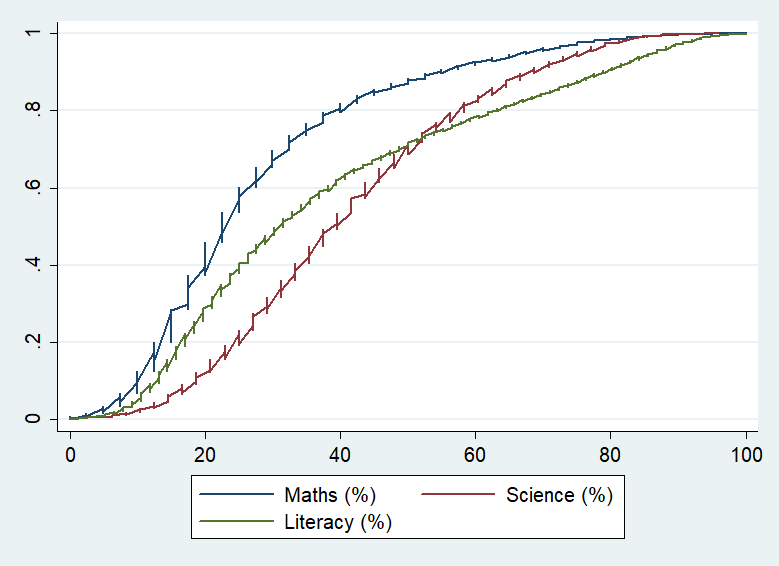
\includegraphics[width=0.4\linewidth]{./results/graphs/figure} \end{center}
\centering
{\footnotesize Source: Own calculations in Stata using 2004 Grade 6 Intermediate Phase Systemic Evaluation.}
\end{figure}

\normalsize

Again, you can reference the figure in-text: figure \ref{fig:1} is a
figure and it displays etc. etc. etc.

This is an organic figure generated with an R chunk that is executed
when the document is knitted (the image is also saved in the folder
\texttt{final-article-template\_files}):

\begin{center}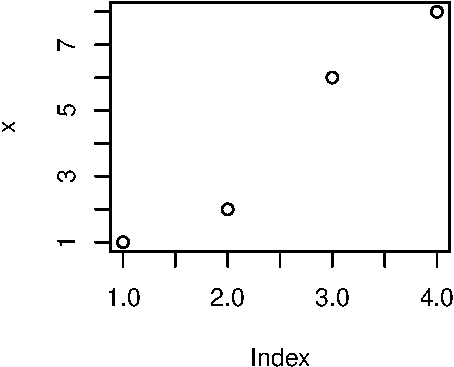
\includegraphics[width=0.4\linewidth]{final-msc-article_files/figure-latex/unnamed-chunk-2-1} \end{center}

Regarding R chunks: If you want a chunk's code to be printed, include
set \texttt{echo\ =\ TRUE}. \texttt{message\ =\ FALSE} stops R printing
package loading details and setting \texttt{warning\ =\ FALSE} should
suppress most warnings.

\newpage

\section{\texorpdfstring{Recommendations for Further Research
\label{Recom}}{Recommendations for Further Research }}\label{recommendations-for-further-research}

\newpage

\section{\texorpdfstring{Concluding Remarks
\label{Concl}}{Concluding Remarks }}\label{concluding-remarks}

\newpage

\section{References}\label{references}

\hypertarget{refs}{}
\hypertarget{ref-Brinton2014}{}
Brinton, C. G. \emph{et al.} (2014) `Learning about social learning in
MOOCs: From statistical analysis to generative model', \emph{IEEE
Transactions on Learning Technologies}. IEEE, 7(4), pp. 346--359. doi:
\href{https://doi.org/10.1109/TLT.2014.2337900}{10.1109/TLT.2014.2337900}.

\hypertarget{ref-Stadtfeld2019}{}
Stadtfeld, C. \emph{et al.} (2019) `Integration in emerging social
networks explains academic failure and success', 116(3), pp. 792--797.
doi:
\href{https://doi.org/10.1073/pnas.1811388115}{10.1073/pnas.1811388115}.

\newcommand\wordcount{
    \immediate\write18{texcount -sub=section \jobname.tex  | grep "Section" |     sed -e 's/+.*//' | sed -n \thesection p > 'count.txt'}
(\input{count.txt}words)}

\section*{References}

\end{document}
